\section{Evaluation}
\label{sec:Eval}

\subsection{Program Synthesis}

To evaluate our synthesizer, we selected three different cache configurations
and ran our synthesizer on a set of random test cases. For each configuration,
the test cases consist of pairs of a 16-bit address and a block number
appropriate for the configuration. We also experimented with hole depths of 1
and 2. The results are shown in Figure~\ref{Fig:synth_results}.

\begin{figure}[h]
  \centering
  \begin{tabular}{|c|c|c|c|c|}
    \hline
    Configuration & Hole depth & Total test cases & Exact matches & Relative difference
    \\ \hline
    8, 4, 4     & 1 & 64  & 10 & 25.0\% \\
                & 2 & 64  & 25 & 21.9\% \\ \hline
    16, 8, 4, 4 & 1 & 128 & 15 & 7.81\% \\
                & 2 & 128 & 17 & 10.9\% \\ \hline
    8, 8, 8, 8  & 1 & 128 & 15 & 50.0\% \\
                & 2 & 128 & 23 & 25.0\% \\ \hline
  \end{tabular}
  \caption{Cache configurations used with the synthesizer. The configuration
    column corresponds to the cache sizes used. Exact matches corresponds to the
    number of actual blocks matching expected blocks. Relative difference is the
    total deviation in the actual distribution of homed caches from the expected
    distribution of homed caches.}
  \label{Fig:synth_results}
\end{figure}

Note that increasing the depth tends to sometimes, but not always, decrease the
relative difference rate. However, this comes at the cost of expanding the
search space. There also need to be enough random test cases to cover all blocks
and addresses in the configuration, or the synthesizer will risk overfitting
like in machine learning approaches. For example, if all test cases end up
having addresses less than some amount $N$, then the resulting hash function may
not select the higher-valued bits of $N$.

This project made us realize that coming up with a good objective function and
search strategy is very difficult. As can be observed in the table, the
objective function of simply matching up blocks is not a good fit for the
synthesis task. For example, the 8, 8, 8, 8 depth 1 configuration achieves a
relative difference of 50\% and would be completely outclassed by a simple
hashing scheme. We also tried an objective function that minimizes the absolute
difference, but we did not find a way to make it efficient enough to terminate
within a reasonable amount of time. Future work could include optimizing the
helper functions to be more amenable to logical encoding, devising a better
objective function, and integrating machine learning techniques to improve the
search strategy.

The sketch was comparably easier to construct than the objective function, but
there is still room for improvement. We currently treat the sketch as a black
box binary function, but we could incorporate aspects from more interesting hash
functions like the parameterized hash function approach we have described in
this report.

\subsection{Parameterized Hash Functions}

For the voting algorithm, we approached simulation by treating all of the
numbers in the ranges of $[0, 2^{8}]$ and $[0, 2^{16}]$ as memory addresses and
hashing them against a simple array of 4 caches of sizes 3, 2, 2, and 1.  While
we tested mainly with this setup, the number of caches and their sizes are
easily configurable.  The graphs below show the histograms of the homed data,
namely, the number of addresses in the space that were mapped to the given
cache.  Ideally, we expect the number of addresses in each cache to follow the
3, 2, 2, 1 distribution.  The metrics chosen were the modulo scheme, the sum of
positive bits, and addition of the median number of caches.

\begin{figure}[h]
  \centering
  \begin{minipage}[b]{0.4\textwidth}
    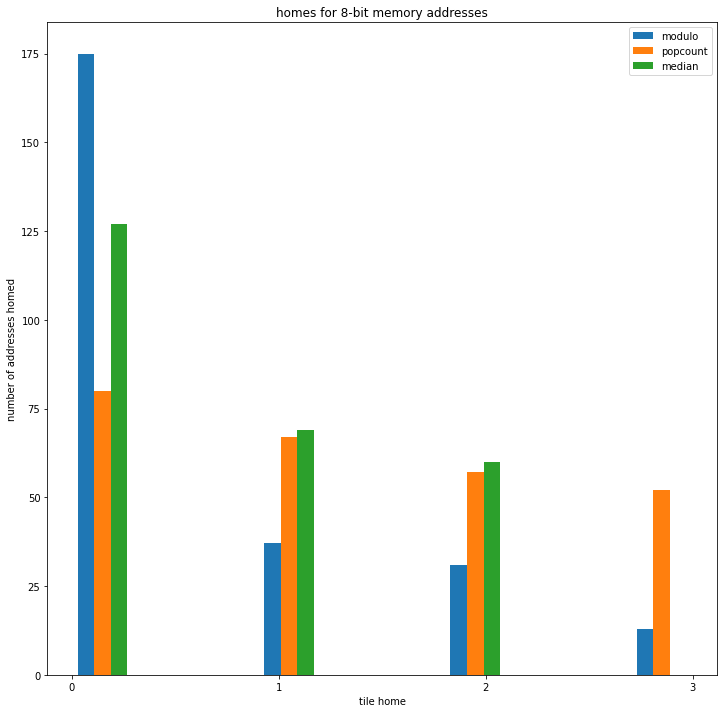
\includegraphics[width=\textwidth]{homes.png}
    \caption{256 bit memory space}
    \label{Fig:homes}
  \end{minipage}
  \hfill
  \begin{minipage}[b]{0.4\textwidth}
    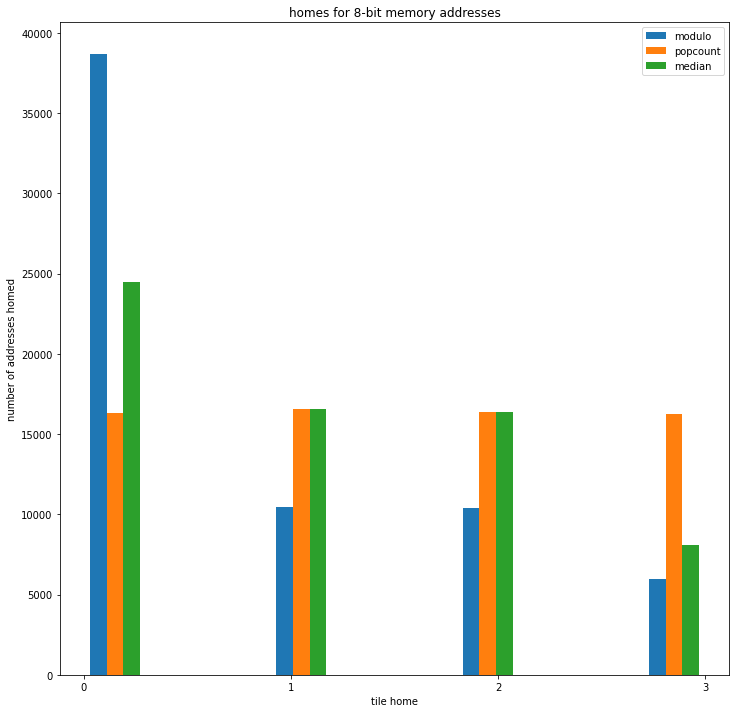
\includegraphics[width=\textwidth]{homes2.png}
    \caption{65536 bit memory space }
    \label{Fig:homes2}
  \end{minipage}
\end{figure}

From the graphs we can see first that popcount is not a good metric for deciding
homes as it collapses to the uniform distribution with enough data.
Interestingly, the remaining two approaches, modulo and median, do roughly match
the distribution of cache sizes, with most data going to the default largest
cache, less going to the middle two largest caches, and the least going to the
smallest cache.  The median performs much closer to the ground truth, however it
is not clear what this intuitively captures about the data.  Finally, the modulo
scheme seems to unduly weight the largest cache, but as it roughly captures the
relative caches sizes, we might be able to temper this somehow.  While these
weighting schemes don't quite capture the distribution exactly, it is clear that
they can be modified to provide a more robust picture of the cache size
distributions.

There are a number of improvements that we could make as a second pass in
hardening this approach.  The number and sizes of caches should be changed
widely, and the sizes of the caches should be powers of 2, or simple arithmetic
combinations of powers of 2, to mimic real world conditions. As noted
previously, the weighting function is crucial to observing a smooth distribution
matching the cache sizes.  The options we tried should be expanded to find
better matches.

Finally, the hash function we used was the Pearson function, which is
traditionally based on a 256-bit table of randomized seed values.  To minimize
the impact of this on memory in a production many-core system, this can be
replaced with alternative metrics, such as a subtraction of the memory address
from 256. Ultimately, however, we can conclude that the above schemes, both
synthesis and voting, are flexible and highly configurable approaches to
parameterizing cache-based hash functions.
